\documentclass[a5paper]{article}
\usepackage{graphicx}
\usepackage{hyperref}
\usepackage[final]{pdfpages}
\usepackage[parfill]{parskip}% don't indent new sections
\usepackage[utf8]{inputenc}
\usepackage{listings}
\usepackage{color}
\usepackage[a4paper]{geometry}
\pagestyle{empty}

\definecolor{dkgreen}{rgb}{0,0.6,0}
\definecolor{gray}{rgb}{0.5,0.5,0.5}
\definecolor{mauve}{rgb}{0.58,0,0.82}

\lstset{frame=tb,
    language=Java,
    aboveskip=3mm,
    belowskip=3mm,
    showstringspaces=false,
    columns=flexible,
    basicstyle={\small\ttfamily},
    numbers=left,
    numberstyle=\tiny\color{gray},
    keywordstyle=\color{blue},
    commentstyle=\color{dkgreen},
    stringstyle=\color{mauve},
    breaklines=true,
    breakatwhitespace=true,
    tabsize=3
}

\title{Practical Concurrent and Parallel Programming}
\author{Emil Lynegaard}

\begin{document}

\includepdf[pages=1]{res/front_page.pdf}
\maketitle
\textit{I hereby declare that I have answered thede exam questions myself without any outside help.}\\

Through all tests, the same machine will be used. Below are the results of \texttt{SystemInfo}:


\begin{table}[!ht]
\begin{center}
\begin{tabular}{ l l }
OS & Linux; 4.13.12-1-ARCH; amd64\\
JVM & Oracle Corporation; 1.8.0\_144\\
CPU & null; 8 "cores"\\
Date & 2017-12-11T09:20:13+0100
\end{tabular}
\end{center}
\caption{System Info}
\label{sysinfo}
\end{table}

\section{Question 1}
\subsection{}
Seeing as we are interested in seeing how well each implementation performs on random input of different sizes, we use Mark9 for the benchmarking, as it calculates the per element mean time and standard deviation.

\begin{figure}[!ht]
    \centering
    \noindent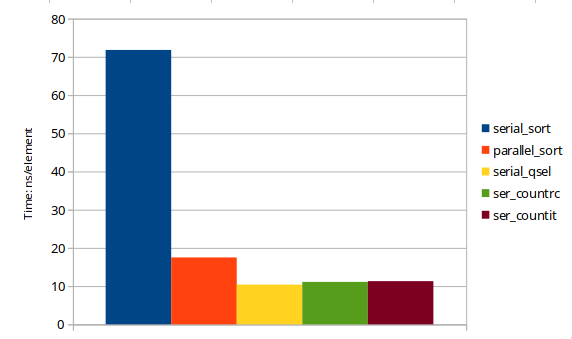
\includegraphics[scale=0.5]{res/graph_q1.png}
    \caption{Plot of running times of given implementations. Tested with size = 10000000.}
    \label{fig:graphq1}
\end{figure}

From graph \ref{fig:graphq1} we see that, perhaps unsurprisingly, the serial quickselect and quickcount implementations beat out serial sort entirely.
We do however see parallel sort get rather close to the expected linear running time implementations, due to the test machine having a quad-core CPU,
allowing an approximate 4 time speedup from the serial implementation. Between the expected linear running time algorithms, it seems serial quickselect 
beat out its quickcount counterparts, however the difference is so small that we have yet to find a definitive winner.

\subsection{}


\section{Question 2}
\subsection{}
\begin{lstlisting}
      (int) Arrays.stream(inp).skip(1).filter(i -> i < p).count();
\end{lstlisting}
Where \texttt{inp} is our input array, and \texttt{p} is our current partition candidate.
Skip the first element as this is the index of the partition element with which we do not wish to compare.

\subsection{}
\begin{lstlisting}
          Arrays.stream(inp).skip(1).filter(i -> i < p).toArray();
          Arrays.stream(inp).skip(1).filter(i -> i >= p).toArray();
\end{lstlisting}

\subsection{}
\begin{lstlisting}
public static int quickCountStream(int[] inp) {
    int partition=-1, count=0, n=inp.length;
    int target = n/2;
    do {
        partition=inp[0];
        final int p = partition;
        n=inp.length;
        count = (int) Arrays.stream(inp).skip(1).filter(i -> i < p).count();
        if (count == target) break;
        if (count > target){
            inp = Arrays.stream(inp).skip(1).parallel.()filter(i -> i < p).toArray();
        }else{
            inp = Arrays.stream(inp).skip(1).parallel().filter(i -> i >= p).toArray();
            target=target-count-1;
        }
    } while( true );
    return partition; // we are on target
}
\end{lstlisting}

Combining the two we get above implementation, which yields correct results.

\subsection{}
\begin{lstlisting}
    Arrays.stream(inp).parallel().skip(1).filter(i -> i < p).count();
    Arrays.stream(inp).parallel().skip(1).filter(i -> i < p).toArray();
    Arrays.stream(inp).parallel().skip(1).filter(i -> i >= p).toArray();
\end{lstlisting}
Here we simply throw \texttt{.parallel()} onto the pipelines from before.

\subsection{}

\begin{lstlisting}
public static int quickCountStream(int[] inp) {
    int partition=-1;
    int target = inp.length/2;
    // Since we have to be working with boxed Integers. We start off by converting.
    List<Integer> list = Arrays.stream(inp).boxed().collect(Collectors.toList());
    do {
        partition = list.get(0);
        final Integer p = partition;
        Map<Boolean, List<Integer>> res = list.stream().skip(1).parallel()
            .collect(Collectors.partitioningBy(i -> i < p));

        List<Integer> smaller = res.get(true);
        System.out.println(Arrays.toString(smaller.toArray()));
        List<Integer> bigger = res.get(false);
        System.out.println(Arrays.toString(bigger.toArray()));

        if (smaller.size() == target) break;
        if (smaller.size() > target) list = smaller;
        else {
            target=target-smaller.size()-1;
            list = bigger;
        }
   } while( true );
    return partition; // we are on target
}
\end{lstlisting}
To avoid having to constantly do boxing, since Collectors does not work with primitives,
we start off by converting our \texttt([] inp) to \texttt{List<Integer>}.

The \texttt{partitioningBy} collector gives us a map of all with two entries.
The \texttt{true} entry on line 12, holding all elements larger than our partition element, and false entry on line 14 holding
all the elements larger than or equal to our partition element. The size of \texttt{smaller} now represents our \texttt{count}
from before, and the remainder of the code is similar to the given code.

\subsection{TODO} 

\section{Question 3 - TODO}
By initially deciding what ranges threads will work on for the entire algorithm, we risk a thread winding up
with a range of the input that we can discard as useless after a single iteration. 

\section{Question 4}
\subsection{}
We are not guaranteed to always grab locks in the same order, hence we are prone to dead-locks.

\subsection{}

\begin{lstlisting}
union(0,1)
union(1,0)
\end{lstlisting}

Above example when executed in parallel may lead to the first call grabbing the lock on \texttt{nodes[0]}, the second call grabbing the lock on \texttt{nodes[1]} and both calls thereafter waiting to get the lock on the node that their counterpart already grabbed.

\subsection{}
We modify the given \texttt{concurrent()} method in class \texttt{UnionFindTest} in file \texttt{MyUnionFind.java} to target the issue we identified in 4.1.
\begin{lstlisting}
public void deadlock(final int size, final UnionFind uf) throws Exception {
    final int[] numbers = new int[size];
    for (int i = 0; i < numbers.length; ++i) numbers[i] = i;
    final int threadCount = 32;
    final CyclicBarrier startBarrier = new CyclicBarrier(threadCount+1), 
          stopBarrier = startBarrier;
    Collections.shuffle(Arrays.asList(numbers));
    for (int i = 0; i < threadCount; ++i) {
        final boolean reverse = i%2==0;
        Thread ti = new Thread(new Runnable() { public void run() {
            try { startBarrier.await(); } catch (Exception exn) { }
            if (reverse)
                for (int j=0; j<100; j++)
                    for (int i = 0; i < numbers.length - 1; ++i) 
                        uf.union(numbers[i], numbers[i + 1]);
            else 
                for (int j=0; j<100; j++)
                    for (int i = 0; i < numbers.length - 1; ++i) 
                        uf.union(numbers[i + 1], numbers[i]);
            try { stopBarrier.await(); } catch (Exception exn) { }
        }});
        ti.start();
    }
    startBarrier.await();
    stopBarrier.await();
    final int root = uf.find(0);
    for (int i : numbers) {
        assertEquals(uf.find(i), root);
    }
    System.out.println("No deadlocks");
}
\end{lstlisting}

As seen from line 10 to 20, half the threads will now be attempting to union nodes in reverse order of the other half.
From my tests, calling the above defined \texttt{deadlock} method with parameters shown below, deadlocked every time.

\begin{lstlisting}
UnionFindTest test = new UnionFindTest();
test.deadlock(itemCount, new BogusFineUnionFind(itemCount));
\end{lstlisting}

By merely adding a check to the given \texttt{union()} method in class \texttt{BogusFineUnionFind} to ensure we always lock the lowest entry of the \texttt{nodes} array first, the deadlock test
executes without deadlocking.

\section{Question 5}

\end{document}
